% Chapter 3

\chapter{System Overview} % Main chapter title

\label{systemoverview} % For referencing the chapter elsewhere, use \ref{Chapter1} 

\lhead{Chapter 3. \emph{System Overview}} % This is for the header on each page - perhaps a shortened title

%----------------------------------------------------------------------------------------

\section{Introduction}

The Context-Aware Guide (subsequently called "CA Guide") needs to be defined to fit indoor and outdoor exhibitions, like classical museums, parks and gardens. 
The basic functionality must be accessible even by persons not familiar with mobile technology. The context awareness techniques can help avoid big parts of explicit user input.

The following figure shows an overview of the complete system, consisting of a museum guide front-end running on a mobile device, a back-end for the configuration of the guide and performing analytic functions. A database server is accessed by both system parts and represents the communication basis - there is no direct communication between font and back end. All data is exchanged over the database, enabling asynchronous communication.

As database server Couchbase was choosen due to it's automatic synchronization capabilities, it's mobile version and it's ability to scale out without completely redesigning the way the database is accessed by the application.\footnote{After actually having reached the limits of scalabity of a single classical relational database server of a commercial project and painfully distributing the database on several servers of the productive system, the idea of an easy scale out using a document based database and map-reduce queries seemed even more ingenious to me.} 

\begin{figure}[H]
\centering
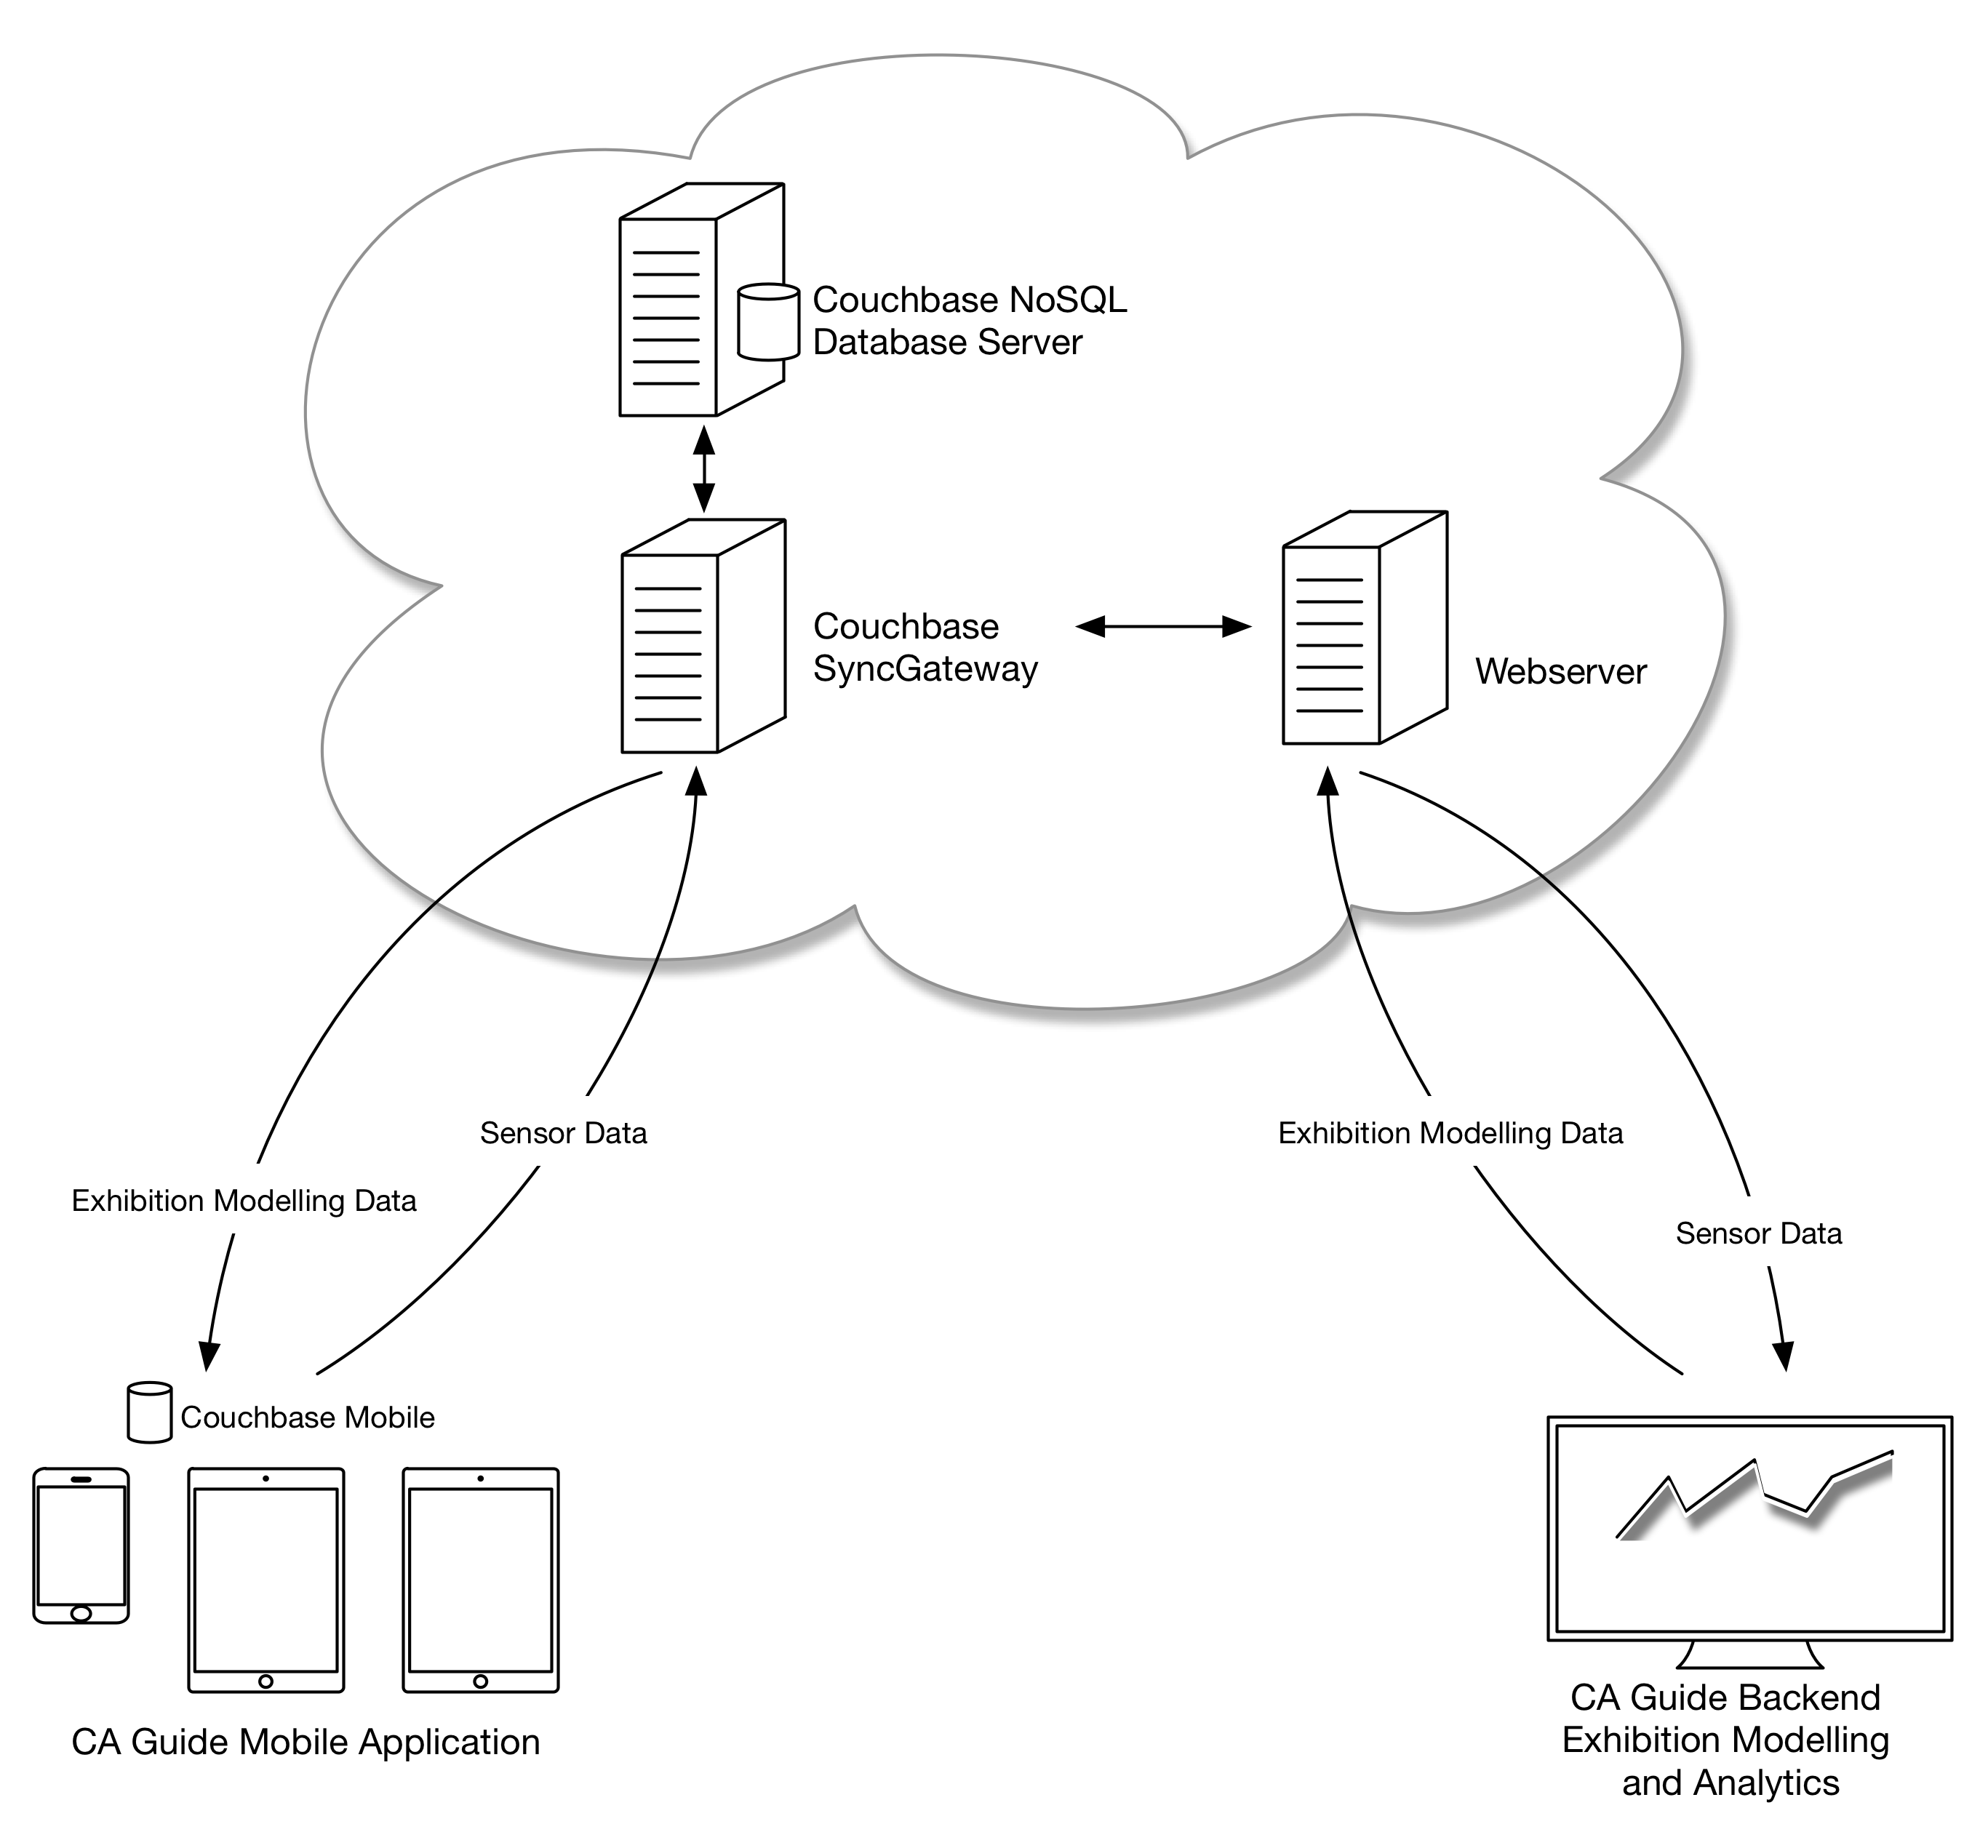
\includegraphics[height=0.8\textwidth]{system-overview}
\caption{CA Guite Architecture Overview}
\end{figure}

Image Mockup CA Guide 

Image A Backend Screen Mockup

\section{Data Structure}

\subsection{Exhibition Modelling}

A single exhibition is modeled in the JSON data format. Compared to XML, JSON is more readable and easier to produce without dedicated tools in a simple text editor.

The entities needed for modelling an exhibition are:

Image entyty relationship diagram

With a normal relational database, pretty much of the entities would be saved in separate tables using primary keys and foreign keys to represent the relationships between the tables.

In a document-oriented database the whole exhibition can be stored in an aggregated way. 

\begin{lstlisting}
key: "exhibition-CXN01"
value: {
 "type":"exhibition",
 "city":"Konstanz",
 "pois": [{
	 "name":"Dom", 
	 "locationDefinition": {
	 	"type": "circle",
	 	"location": [15.0020312,2.3434322],
	 	"radius": 30,
	 	"floor": 1
	 }, 
	 "text":"", 
	 "images":[], 
	 "audio":{
	 	"level1":
	 	"level2":
	 	"level3":
	 }, 
	 "videos":[]},]
}
\end{lstlisting}

A JSON Schema is used for asserting a valid structure of a JSON file, similar to a DTD (Data Type Definition) in XML (http://json-schema.org).

\subsection{Sensor Data}

Sensor data is saved to the Couchbase database to allow replaying it for development, testing, presentations and for analytics presented in the system's web backend. 

The single measurements can be very high frequent, for example in case of accelerometer data, that is updated every 10 millisecons. New beacon measurements are available every second. Events on a higher logical level, like "entering region a", will occur less frequently.

\begin{lstlisting}[basicstyle=\footnotesize]
key: SENSORTRACE-CXN01
value: {
  "date": "2015-02-12",
  "time": "20:15",
  "accelerometer": [
    {"timestamp": 12345678.35, "data": [1.235, 0.364, 0.021]},
    {"timestamp": 12345678.40, "data": [1.217, 0.378, 0.009]},
    ...
  ],
  "gyroscope": [
    {"timestamp": 12345678.35, "data": [1.235, 0.364, 0.021]},
    {"timestamp": 12345678.40, "data": [1.217, 0.378, 0.009]},
    ...
  ],
  "magnetometer": [
    {"timestamp": 12345678.35, "data": [1.235, 0.364, 0.021]},
    {"timestamp": 12345678.40, "data": [1.217, 0.378, 0.009]},
    ...
  ],
  "beacons": [
    {"timestamp": 12345679.05, "data": [["A3F3", -51],["85B7", -68]]},
    {"timestamp": 12345680.05, "data": [["A3F3", -51],["85B7", -68]]},
    ...
  ],
  "gps": [
    {"timestamp": 12345679.35, "data": [1.44, 10.021]},
    {"timestamp": 12345680.36, "data": [1.44, 10.009]},
    ...
  ],
}
\end{lstlisting}


\section{Setting up the Couchbase Server Infrastructure}

Couchbase Server
Admin Port

Couchbase Sync Gateway
config.json

%Backend has two databases, work in progress in couchbase NoSQL, aggregates site area beacon, site aggregate published over sync-gateway